\documentclass[10pt,a4paper]{article}
\usepackage[UTF8,fontset = windows]{ctex}
\setCJKmainfont[BoldFont=黑体,ItalicFont=楷体]{华文中宋}
\usepackage{amssymb,amsmath,amsfonts,amsthm,mathrsfs,dsfont,graphicx}
\usepackage{ifthen,indentfirst,enumerate,color,titletoc}
\usepackage{tikz}
\usepackage{makecell}
\usepackage{longtable}
%\usepackage{mathptmx}

\usetikzlibrary{arrows,calc,intersections,patterns,decorations.pathreplacing,angles,quotes}
\usepackage[bf,small,indentafter,pagestyles]{titlesec}
\usepackage[top=1in, bottom=1in,left=0.8in,right=0.8in]{geometry}
\renewcommand{\baselinestretch}{1.65}
\newtheorem{defi}{定义~}
\newtheorem{eg}{例~}
\newtheorem{ex}{~}
\newtheorem{rem}{注~}
\newtheorem{thm}{定理~}
\newtheorem{coro}{推论~}
\newtheorem{axiom}{公理~}
\newtheorem{prop}{性质~}
\newcommand{\blank}[1]{\underline{\hbox to #1pt{}}}
\newcommand{\bracket}[1]{(\hbox to #1pt{})}
\newcommand{\onech}[4]{\par\begin{tabular}{p{.9\textwidth}}
A.~#1\\
B.~#2\\
C.~#3\\
D.~#4
\end{tabular}}
\newcommand{\twoch}[4]{\par\begin{tabular}{p{.46\textwidth}p{.46\textwidth}}
A.~#1& B.~#2\\
C.~#3& D.~#4
\end{tabular}}
\newcommand{\vartwoch}[4]{\par\begin{tabular}{p{.46\textwidth}p{.46\textwidth}}
(1)~#1& (2)~#2\\
(3)~#3& (4)~#4
\end{tabular}}
\newcommand{\fourch}[4]{\par\begin{tabular}{p{.23\textwidth}p{.23\textwidth}p{.23\textwidth}p{.23\textwidth}}
A.~#1 &B.~#2& C.~#3& D.~#4
\end{tabular}}
\newcommand{\varfourch}[4]{\par\begin{tabular}{p{.23\textwidth}p{.23\textwidth}p{.23\textwidth}p{.23\textwidth}}
(1)~#1 &(2)~#2& (3)~#3& (4)~#4
\end{tabular}}
\begin{document}
\begin{enumerate}[1.]

\item 把下列指数式写成对数式:\\
(1) $10^{-2}=0.01$:\blank{50};\\
(2) $(\dfrac 12)^0=1$:\blank{50};\\
(3) $5^x=6$:\blank{50}.
\item 把下列对数式写成指数式:\\
(1) $x=\log _{16}32$:\blank{50};\\
(2) $\log _{\pi }x=4$:\blank{50};\\
(3) $\log _x9=2$:\blank{50}.
\item 求下列各式中的$x$:\\
(1) $\log _{\frac 12}x=3$, $x=$\blank{50};\\
(2) $\log _3\dfrac 1{27}=x$, $x=$\blank{50};\\
(3) $\log _{100}1000=x$, $x=$\blank{50};\\
(4) $\log _x16=4$, $x=$\blank{50}.
\item 计算: $\log _55\sqrt 5+\ln e$.
\item 计算: $\lg \sqrt {10}-\lg 0.01$.
\item 计算: $\log _{12}6+\log _{12}2$.
\item 计算: $\log _348-4\log _32$.
\item 用$\log _aM$、$\log _aN$表示$\log _aMN^2$.
\item 用$\log _aM$、$\log _aN$表示$\log _a\dfrac{\sqrt M}N$.
\item 计算: $3^{\log _31}+\log _248-\log _23$.
\item 计算: $2\log _7\dfrac{35}9+4\log _73+2\log _7\dfrac 1{10}+\log _74$.
\item 计算: $\log _32\times \log _53\times \log _85$.
\item 计算: $(\log _43+\log _83)\times \log _32$.
\item 计算: $\log _2\dfrac 1{49}\times \log _3\dfrac 1{16}\times \log _7\dfrac 1{27}$.
\item 计算: $\log _ab\cdot \log _bc\cdot \log _ca$.
\item 计算: $(\log _43+\log _83)(\log _32+\log _94)$.
\item 已知$\log _32=m$, 试用$m$表示$\log _{32}18$.
\item 已知$\lg 2=a$, $\lg 3=b$.\\
(1) 求$\lg 5$;\\
(2) 求$\log _23$;\\
(3) 求$\log _{12}25$.
\item 求出下列各式中$x$的取值范围: ($a>0$且$a\ne 1$)\\
(1) $\log _a(x^2+1)$;\\
(2) $\log _a(x-2)$;\\
(3) $\log _a\dfrac 1{x+2}$.
\item 在下列各式中的横线上填入适当的值, 使等式成立:\\
(1) $\log _5$\blank{20}$=1$;\\
(2) $2^{\log _31}=$\blank{20};\\
(3) $(\dfrac 15)^{\log _{0.2}3}=$\blank{20};\\
(4) $\sqrt 3^{\log _{\sqrt 3}}$\blank{20}$=7$.
\item 用$\log _ax$、$\log _ay$、$\log _a(x+y)$、$\log _a(x-y)$表示下列各式:\\
(1) $\log _a(x^2-y^2)$;\\
(2) $\log _4\dfrac{x^3y}{(x+y)^4}$;\\
(3) $\log _a(\dfrac{\sqrt x}{\sqrt y}-\dfrac{\sqrt y}{\sqrt x})$.
\item 计算: $\log _2(\log _216)$.
\item 计算: $2^{\log _65}\times 3^{\log _65}$.
\item 计算: $\sqrt {\lg^25-2\lg 5+1}$.
\item 计算: $\lg ^25+\lg ^2\times \lg 50$.
\item 设$56^a=14$, 试用$a$表示$\log _756$.
\item 已知$5.4^x=3$, $0.6^y=3$, 求$\dfrac 1x-\dfrac 1y$的值.
\item 已知函数$f(x)=x^2-4x-5$, $x\in [1,3]$, 判断其是否存在反函数. 若存在, 求出反函数; 若不存在, 说明理由.
\item 求函数$y=-x^3$的反函数.
\item 求函数$y-\dfrac x{x+2}$的反函数.
\item 求函数$y=x^2+1$($x<0$)的反函数.
\item 已知$f(x)=1-x^2$($x<-1$), 求$f^{-1}(-3)$的值.
\item 已知函数$y=\dfrac a{x+1}$的反函数的图像经过点$(\dfrac 12,1)$, 求实数$a$的值.
\item 已知函数$y=f(x)$的图像与函数$y=\dfrac{x-1}{x+1}$的图像关于直线$y=x$对称, 求函数$y=f(x)$的解析式.
\item 判断题: (正确的在括号内用``$\checkmark$''表示, 错误的用``$\times$''表示)\\
(1) 存在反函数的函数一定是单调函数.\blank{20};\\
(2) 偶函数存在反函数.\blank{20};\\
(3) 奇函数必存在反函数.\blank{20}.
\item 一次函数$y=-x$的图像与它的反函数的图像重合. 试写出一个非一次函数的函数, 使它的图像与其反函数的图像重合.
\item 如果函数$y=f(x)$的图像过点$(0, 1)$, 那么函数$y=f^{-1}(x)+2$的反函数的图像过点\bracket{20}.
\fourch{$(3, 0)$}{$(0, 3)$}{$(1, 2)$}{$(2, 1)$}
\item 如果$y=-\sqrt {1-x^2}$的反函数是$y=-\sqrt {1-x^2}$, 那么原来的函数的定义域可以是\bracket{20}.
\fourch{$(0,+\infty)$}{$[-1,1]$}{$[-1,0]$}{$[0,1]$}
\item 求函数$y=\begin{cases} -\sqrt x, & 0\le x\le 1, \\ x^2, & -1\le x<0 \end{cases}$的反函数.
\item 求函数$y=\lg (x^2-3x+2)$的定义域.
\item 求函数$y=\dfrac{\sqrt {2x-1}}{\lg x}$的定义域.
\item 求函数$y=\sqrt {\lg x}+\lg (5-2x)$的定义域.
\item 求函数$y=10^x+1$的反函数.
\item 求函数$y=\log _2(x+1)$的反函数.
\item 求函数$y=\log _22x$的反函数.
\item 已知函数$f(x)=a^x+b$的图像经过点$(1, 7)$, 反函数$f^{-1}(x)$的图像经过点$(4, 0)$, 求函数$f(x)$的表达式.
\item 若$\log _a0.2<\log _a0.1$成立, 求$a$的取值范围.
\item 若$\log _a\pi >\log _a\mathrm{e}$成立, 求$a$的取值范围.
\item 若$\log _a3<0$成立, 求$a$的取值范围.
\item 已知$1<x<2$, $a=2^x$, $b=\log _{0.5}x$, $c=\sqrt x$, 比较$a$、$b$、$c$的大小, 并说明理由.
\item 声音强度$D$(分贝)由公式$D=10\lg (\dfrac I{10^{-16}})$给出, 其中$I(\text{W}/\text{cm}^2)$为声音能量.能量小于$10^{-16}\text{W}/\text{cm}^2$时, 人听不见声音.能量大于$60$分贝属于噪音, 其中$70$分贝开始损害听力神经, $90$分贝以上就会使听力受损, 而一般的人呆在$100$分贝$-120$分贝的空间内, 一分钟就会暂时性失聪.\\
(1) 求人低声说话$I=10^{-13}\text{W}/\text{cm}^2$的声音强度;\\
(2) 求噪音的能量范围;\\
(3) 当能量达到多少时, 人会暂时性失聪?
\item 判断函数$y=\lg\dfrac{x+1}{x-1}$的奇偶性.
\item 设$a>0$且$a\ne 1$, 比较$\log _a2a$与$\log _a3a$的大小.
\item 求证: $y=\lg(1-x)$在定义域上单调递减.
\item 求函数$y=\log _{\frac 15}(x^2-6x+10)$在区间$[1,2]$上的最大值.
\item 解方程$2^{1-x}=\dfrac 1{32}$.
\item 解方程$3^{-x+2}=9^x$.
\item 解方程$4^{2x-1}=1$.
\item 解方程$0.38\cdot 10^{x-3}=0.5$(精确到$0.01$).
\item 解指数方程$2^{x^2+3}=(\dfrac 14)^{\frac 72}$.
\item 解指数方程$9^x-8\cdot 3^x-9=0$.
\item 已知关于$x$的方程$2a^{2x-2}-7a^{x-1}+3=0$有一个根是$x=2$, 求$a$的值并求方程的其余的根.
\item 某种放射性物质不断衰减, 若每经过一年剩留的物质是原来的$\dfrac 45$, 经过多少年, 剩余物质是原来的$\dfrac{64}{125}$?
\item 解方程: $9^x+4^x=\dfrac 52\cdot 6^x$.
\item 解方程: $4^x+4^{-x}-6(2^x+2^{-x})+10=0$.
\item 动物尸体内$^{14}C$的含量每年衰减$0.012\%$, 设动物死亡的时刻$t=0$时, $^{14}C$含量为$100\%$.\\
(1) 写出$^{14}C$含量$y$关于时间$t$的函数解析式;\\
(2) $^{14}C$含量减少到$50\%$需多少时间? (精确到$1$年)
\item 解方程$\log _3(x-2)=1$.
\item 解方程$\log _2(x^2-3x)=2$.
\item 解方程$\log _2(\log _5x)=1$.
\item 解方程$\log _5(x+1)-\log _{\frac 15}(x-3)=1$.
\item 解方程$\log _2^2x+3\log _2x+2=0$.
\item 解方程$\log _x(x^2-x)=\log _x2$.
\item 解方程$\log _{\frac 12}(9^{x-1}-5)=\log _{\frac 12}(3^{x-1}-2)-2$.
\item 解方程$(\lg x)^2-\lg x^2=3$.
\item 解方程: $x^{\log _2x}=32x^4$.
\item 求方程$\log _2(x+4)=(\dfrac 13)^x$根的个数, 并说明理由.
\item 若$x^5=3$, 则$x=$\blank{50}; 若$5^x=3$, 则$x=$\blank{50}.
\item 计算: $\log _236-2\log _23=$\blank{50}.
\item 若$\log _ab\cdot \log _5a=3$, 则$b=$\blank{50}.
\item 函数$y=\log _2x(x\ge 1)$的反函数是\blank{50}.
\item 若点$(1, 7)$既在函数$y=\sqrt {ax+b}$的图像上, 又在其反函数的图像上, 则数对$(a,b)$为\blank{50}.
\item 若$f(x)=3^x+5$, 则$f^{-1}(x)$的定义域是\bracket{20}.
\fourch{$(0,+\infty)$}{$(5,+\infty)$}{$(8,+\infty)$}{$(-\infty ,+\infty)$}
\item 若$\log _{18}9=a$, $18^b=5$, 则$\log _{36}45$等于\bracket{20}.
\fourch{$\dfrac{a+b}{2+a}$}{$\dfrac{a+b}{2-a}$}{$\dfrac{a+b}{2a}$}{$\dfrac{a+b}{a^2}$}
\item 已知函数$f(x)=\dfrac{ax+1}{x-3}$的反函数是$f(x)$本身, 求实数$a$的值.
\item 作出函数$y=\log _2(x-1)$的图像.
\item 作出函数$y=|\log _2(x-1)|$的图像.
\item 已知$\lg x+\lg y=2$, 求$\dfrac 1x+\dfrac 1y$的最小值.
\item 解方程: $4^x+2^{x+1}=80$.
\item 解方程: $\lg (2x+2)+\lg (15-x)=1+\lg 3$.
\item 已知函数$f(x)=\log _a\dfrac{1+x}{1-x}$($a>0$, $a\ne 1$).
(1) 求$f(x)$的定义域;\\
(2) 判断$f(x)$的奇偶性, 并加以证明;\\
(3) 当$a>1$时, 求使$f(x)>0$的$x$的取值范围.
\item 如果光线每通过一块玻璃其强度要减少$10\%$, 求至少需要多少块这样的玻璃重叠起来, 才能使通过它们的光线强度为原来的强度的$\dfrac 13$以下?
\item 如果函数$f(x)=\log _a(-x^2+ax)$的定义域为$(0,\dfrac 12)$, 那么实数$a=$\blank{50}.
\item 如果$45^x=3$, $45^y=5$, 那么$2x+y=$\blank{50}.
\item 若函数$y=f(x)$的图像与函数$y=2^x-1$的图像关于直线$y=x$成轴对称图形, 则函数$y=f(x)$的解析式为\blank{50}.
\item 当$a>1$时, 在同一坐标系中, 函数$y=a^{-x}$与$y=\log _ax$的图像是\bracket{20}.
\fourch{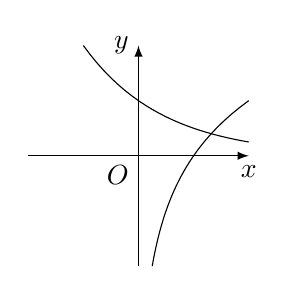
\begin{tikzpicture}[scale = 0.7, >=latex]
    \draw [->] (-2,0) -- (2,0) node [below] {$x$};
    \draw [->] (0,-2) -- (0,2) node [left] {$y$};
    \draw (0,0) node [below left] {$O$};
    \draw [domain = -1:2] plot (\x, {pow(0.5,\x)});
    \draw [domain = -1:2] plot ({pow(0.5,\x)},-\x);
\end{tikzpicture}}
{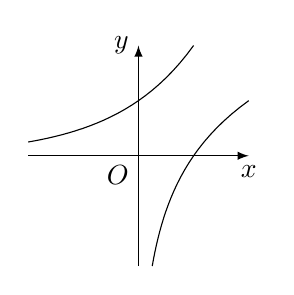
\begin{tikzpicture}[scale = 0.7, >=latex]
    \draw [->] (-2,0) -- (2,0) node [below] {$x$};
    \draw [->] (0,-2) -- (0,2) node [left] {$y$};
    \draw (0,0) node [below left] {$O$};
    \draw [domain = -1:2] plot (-\x, {pow(0.5,\x)});
    \draw [domain = -1:2] plot ({pow(0.5,\x)},-\x);
\end{tikzpicture}}{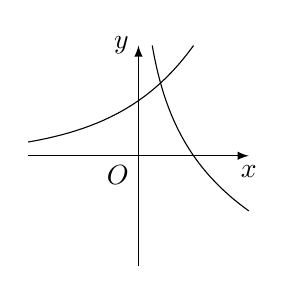
\begin{tikzpicture}[scale = 0.7, >=latex]
    \draw [->] (-2,0) -- (2,0) node [below] {$x$};
    \draw [->] (0,-2) -- (0,2) node [left] {$y$};
    \draw (0,0) node [below left] {$O$};
    \draw [domain = -1:2] plot (-\x, {pow(0.5,\x)});
    \draw [domain = -1:2] plot ({pow(0.5,\x)},\x);
\end{tikzpicture}}{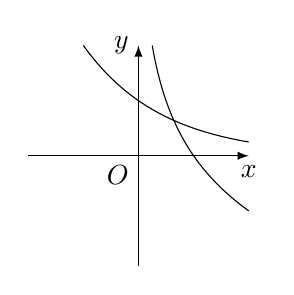
\begin{tikzpicture}[scale = 0.7, >=latex]
    \draw [->] (-2,0) -- (2,0) node [below] {$x$};
    \draw [->] (0,-2) -- (0,2) node [left] {$y$};
    \draw (0,0) node [below left] {$O$};
    \draw [domain = -1:2] plot (\x, {pow(0.5,\x)});
    \draw [domain = -1:2] plot ({pow(0.5,\x)},\x);
\end{tikzpicture}}
\item 函数$f(x)=4+\log _a(x-1)(a>0a\ne 1)$的图像恒经过定点$P$, 则点$P$的坐标是\bracket{20}.
\fourch{$(1, 4)$}{($4, 1)$}{$(2, 4)$}{$(4, 2)$}
\item 已知$0<a<1$, 化简$\sqrt {\lg ^2a-\lg \dfrac{a^2}{10}}$.
\item 已知$\alpha$、$\beta$是方程$\lg ^2x-\lg x-2=0$的两根, 求$\log _{\alpha }\beta +\log _{\beta }\alpha$的值.
\item 判断命题``若函数$y=f(x)$与$y=f^{-1}(x)$的图像有公共点, 则公共点必在直线$y=x$上''的真假, 并说明理由.
\item 如果$^{237}U$在不断的裂变中, 每天所剩留质量与上一天剩留质量相比, 按同一比例减少, 经过$7$天裂变, 剩留的质量是原来的$50\%$, 计算它经过多少天裂变, 剩留质量是原来的$10\%$.


\item 下列各组的两个角中, 终边不相同的一组是\bracket{20}.
\fourch{-$43^\circ$与$677^\circ$}{$900^\circ$与$-1260^\circ$}{$-120^\circ$与$960^\circ$}{$150^\circ$与$630^\circ$}
\item 如果角$\alpha$的终边落在区间$(-3\pi ,-\dfrac{5\pi}2)$内, 那么角$\alpha$所在的象限是\bracket{20}.
\fourch{第一象限}{第二象限}{第三象限}{第四象限}
\item 如果$\alpha$是锐角, 那么$2\alpha$是\bracket{20}.
\fourch{第一象限角}{第二象限角}{小于$180^\circ$的正角}{大于直角的正角}
\item 如果$\alpha$是钝角, 那么$\dfrac{\alpha}2$是\bracket{20}.
\fourch{第一限角}{第二象限角}{第一与第二象限角}{不小于直角的正角}
\item 找出与下列各角终边重合的角$\alpha (0^\circ\le \alpha <360^\circ)$, 并判别下列各角是哪个象限的角:\\
(1) $-1441^\circ$;\\
(2) $1790^\circ$.
\item 把下列各角化成$2k\pi +\alpha$($0\le \alpha <2\pi$, $k\in \mathbf{Z}$)的形式:\\
(1) $\dfrac{50\pi}3$;\\
(2) $-\dfrac{50\pi}3$;\\
(3) $-108^\circ$;\\
(4) $-225^\circ$.
\item 已知扇形的弧长为$\dfrac{5\pi}3$, 半径为$2$, 求扇形的面积$S$及圆心角$\alpha$.
\item 写出终边在$x$轴与$y$轴的夹角的平分线上的角的集合(分别用角度制和弧度制来表示).
\item 在平面直角坐标系中, 用阴影部分表示集合: $\{\alpha|30^\circ+k\cdot 360^\circ\le \alpha \le 60^\circ+k\cdot 360^\circ, \ k\in \mathbf{Z}\}$.
\item 第一象限角的集合是\blank{50}.
\item 终边在坐标轴上的角的集合是\blank{50}.
\item 写出与$60^\circ$终边相同的角的集合$S$, 并写出$S$中适合不等式$-360^\circ\le \alpha <720^\circ$的元素$\alpha$.
\item 写出与$-21^\circ$终边相同的角的集合$S$, 并写出$S$中适合不等式$-360^\circ\le \alpha <720^\circ$的元素$\alpha$.
\item 一条长度等于半径的弦所对的圆心角是多少弧度? 长度分别等于半径的$\sqrt 2$倍和$\sqrt 3$倍的弦所对的圆心角分别是多少弧度?
\item 已知一个直径为$30$厘米的轮子, 每秒旋转$25$弧度, 求轮周上一点在半分钟内所转过的弧长和周数(精确到$0.1$周).
\item 已知角$\alpha$的终边经过点$(3,-4)$, 求角$\alpha$的正弦、余弦和正切的值.
\item 已知角$\alpha$的终边经过点$(-1,-\sqrt 3)$, 求角$\alpha$的正弦、余弦和正切的值.
\item 求$\dfrac{2\pi}3$的六个三角比的值.
\item 求$\dfrac{4\pi}3$的六个三角比的值.
\item 计算: $6\cos 270^\circ+10\sin 0^\circ-4\tan 180^\circ+5\cos 360^\circ$.
\item 计算: $\sin ^2\dfrac{\pi}4-\cos ^2\dfrac{\pi}2+2\tan ^3\dfrac{\pi}4$.
\item 求值: $\sin 1110^\circ$.
\item 求值: $\cos (-\dfrac{7\pi}4)$.
\item 求值: $\tan \dfrac{19\pi}3$.
\item 用判断象限的方法, 确定$\sin 237^\circ$的符号.
\item 用判断象限的方法, 确定$\cos (-390^\circ)$的符号.
\item 用判断象限的方法, 确定$\tan (-\dfrac{7\pi}6)$的符号.
\item 用判断象限的方法, 确定下列式子的符号:
\item 用判断象限的方法, 确定$\tan 135^\circ\cdot \cos 275^\circ$的符号.
\item 用判断象限的方法, 确定$\dfrac{\cos \dfrac{5\pi}6\cdot \tan \dfrac{11\pi}6}{\sin \dfrac{2\pi}3}$的符号.
\item 已知$\sin \theta <0$且$\cos \theta >0$, 确定角$\theta$所在的象限.
\item 已知$\dfrac{\sin \theta}{\tan \theta}>0$, 确定角$\theta$所在的象限.
\item 已知$\alpha$为锐角, 利用三角函数线的有关知识证明: $\sin \alpha <\alpha$.
\item 已知$0<\alpha _1<\alpha _2<\dfrac{\pi}2$, 试利用三角函数的有关知识说明$\sin \alpha _1$与$\sin \alpha _2$的大小, 并判断在$\alpha \in (0,\dfrac{\pi}2)$时, 随着$\alpha$的增大, $\sin \alpha$值的变化趋势.
\item 已知角$\alpha$的终边经过点$P(-2k,3k)$, 且$k<0$, 求$\cos \alpha$与$\csc \alpha$的值.
\item 计算: $\sin (-\dfrac{11\pi}6)+\cos \dfrac{27\pi}7\cdot \tan 4\pi -\cos \dfrac{19\pi}3$.
\item 化简: $m^2\sin (-630^\circ)+n^2\tan (-315^\circ)-2mn\cos (-720^\circ)$.
\item 求三角比$\tan (-\dfrac{\pi}4)$的值.
\item 求三角比$\sin 390^\circ$的值.
\item 求三角比$\sin (-\dfrac{25\pi}2)$的值.
\item 求三角比$\cos (-690^\circ)$的值.
\item 已知$\sin \alpha =-\dfrac 23$, 且$\alpha$是第四象限的角, 求角$\alpha$的其他三角比的值.
\item 已知$\tan \alpha =\dfrac 34$, 且$\alpha$是第三象限的角, 求角$\alpha$的其他三角比的值.
\item 已知$\cos \alpha =\dfrac{12}{13}$, 求$\sin \alpha$、$\tan \alpha$的值.
\item 已知$\cot \alpha =-\dfrac 12$, 求$\sin \alpha$、$\cos \alpha$和$\tan \alpha$的值.
\item 化简: $\dfrac{\sin (\alpha -\pi)\cot (\alpha -2\pi)}{\cos (\alpha -\pi)\tan (\alpha -2\pi)}$.
\item 化简: $\cot ^2\alpha (\tan ^2\alpha -\sin ^2\alpha)$.
\item 已知$\tan x=\sqrt 3$, $x\in [0,2\pi)$, 求角$x$.
\item 已知$\cos x=-\dfrac{\sqrt 2}2$, $x$是第二象限的角, 求角$x$.
\item 证明: $\sin ^4\alpha +\cos ^4\alpha =1-2\sin ^2\alpha \cos ^2\alpha$.
\item 证明: $\tan \alpha -\cot \alpha =\dfrac{1-2\cos ^2\alpha}{\sin \alpha \cos \alpha}$.
\item 证明: $\dfrac{1-2\sin \alpha \cos \alpha}{\cos ^2\alpha -\sin ^2\alpha}=\dfrac{1-\tan \alpha}{1+\tan \alpha}$.
\item 已知$\tan \alpha =2$, 求$\dfrac{\sin \alpha -\cos \alpha}{\sin \alpha +\cos \alpha}$的值.
\item 利用诱导公式, 求角$\dfrac{23\pi}3$和$-\dfrac{87\pi}4$的正弦、余弦、正切的值.
\item 已知$\alpha$是第二象限的角, 化简$\sqrt {\dfrac{1+\sin \alpha}{1-\sin \alpha}}-\sqrt {\dfrac{1-\sin \alpha}{1+\sin \alpha}}$.
\item 证明: $\sin ^2\alpha +\sin ^2\beta -\sin ^2\alpha \sin ^2\beta +\cos ^2\alpha \cos ^2\beta =1$.
\item 证明: $2(1-\sin \alpha)(1+\cos \alpha)=(1-\sin \alpha +\cos \alpha)^2$.
\item 证明: $\dfrac{\tan ^2\alpha -\cot ^2\alpha}{\sin ^2\alpha -\cos ^2\alpha}=\sec ^2\alpha +\csc ^2\alpha$.
\item 求三角比$\cos 105^\circ$的值.
\item 求三角比$\sin 165^\circ$的值.
\item 求三角比$\tan \dfrac{5\pi}{12}$的值.
\item 化简: $\cos (\alpha +\beta)\cos \beta +\sin (\alpha +\beta)\sin \beta$.
\item 化简: $\sin (\theta +105^\circ)\cos (\theta -15^\circ)-\cos (\theta +105^\circ)\sin (\theta -15^\circ)$.
\item 化简: $\cos (\dfrac{\pi}4+\alpha)+\sin (\dfrac{\pi}4+\alpha)$.
\item 化简: $\dfrac{\tan (\alpha -\beta)+\tan \beta}{1-\tan (\alpha -\beta)\tan \beta}$.
\item 化简: $\cos (90^\circ+\alpha)+\sin (180^\circ+\alpha)-\sin (-\alpha)$.
\item 化简: $\dfrac{\sin (\pi -\alpha)}{\tan (\pi +\alpha)}\cdot \dfrac{\cot (\dfrac{\pi}2-\alpha)}{\tan (\dfrac{\pi}2+\alpha)}\cdot \dfrac{\cos (-\alpha)}{\sin (2\pi -\alpha)}$.
\item 证明: $\dfrac{\sin (\alpha +\beta)}{\cos \alpha \cos \beta}=\tan \alpha +\tan \beta$.
\item 证明: $\sin (\alpha +\beta)\cos (\alpha -\beta)=\sin \alpha \cos \alpha +\sin \beta \cos \beta$.
\item 把$\sqrt 3\sin \alpha +\cos \alpha$化成$A\sin (\alpha +\varphi)$($A>0$)的形式.
\item 把$5\sin \alpha -12\cos \alpha$化成$A\sin (\alpha +\varphi)$($A>0$)的形式.
\item 已知$\sin \theta =-\dfrac 7{25}$, $\theta \in (\pi ,\dfrac{3\pi}2)$, 求$\tan (\theta -\dfrac{\pi}4)$的值.
\item 已知$\sin \alpha =\dfrac 8{17}$, $\cos \beta =-\dfrac 5{13}$, $\alpha,\beta \in (\dfrac{\pi}2,\pi)$, 求$\cos (\alpha +\beta)$的值.
\item 在$\triangle ABC$中, 若$\tan A$与$\tan B$是方程$x^2-6x+7=0$的两个根, 求$\tan C$的值.
\item 已知$\sin \alpha =\dfrac 5{13}$, $\cos \beta =-\dfrac 35$, 且$\alpha$、$\beta$都是第二象限的角.求$\sin (\alpha -\beta)$、$\cos (\alpha -\beta)$、$\tan (\alpha -\beta)$的值.
\item 已知$\sin \alpha -\sin \beta =-\dfrac 13$, $\cos \alpha -\cos \beta =\dfrac 12$, 求$\cos (\alpha -\beta)$的值.
\item 已知$\tan \alpha$、$\tan \beta$是方程$x^2+6x+7=0$的两个根, 求证: $\sin (\alpha +\beta)=\cos (\alpha +\beta)$.
\item 已知$(1+\tan \alpha)(1+\tan \beta)=2$, 且$\alpha$、$\beta$都是锐角, 求证: $\alpha +\beta =\dfrac{\pi}4$.
\item 在锐角三角形$ABC$中, 求证: $\tan A+\tan B+\tan C=\tan A\tan B\tan C$.
\item 已知$\cos \varphi =-\dfrac 13$, 且$\pi <\varphi <\dfrac{3\pi}2$, 求$\sin 2\varphi$、$\cos 2\varphi$和$\tan 2\varphi$的值.
\item 已知等腰三角形的底角的正弦值等于$\dfrac 45$, 求这个三角形的顶角的正弦、余弦和正切的值.
\item 已知$\cos \theta =\dfrac 13$, 且$\theta$是第四象限的角, 求$\sin \dfrac{\theta}2$、$\cos \dfrac{\theta}2$和$\tan \dfrac{\theta}2$的值.
\item 已知等腰三角形的顶角的余弦值等于$-\dfrac 7{25}$, 求这个三角形的底角的正弦、余弦和正切的值.
\item 求值: $\tan 15^\circ+\cot 15^\circ$.
\item 求值: $\sin ^4\dfrac{\pi}8+\cos ^4\dfrac{\pi}8$.
\item 证明: $1+\sin \alpha =(\sin \dfrac{\alpha}2+\cos \dfrac{\alpha}2)^2$.
\item 证明: $\dfrac{1+\sin 2\alpha -\cos 2\alpha}{1+\sin 2\alpha +\cos 2\alpha}=\tan \alpha$.
\item 证明: $\dfrac{1+\sin \alpha}{\cos \alpha}=\dfrac{1+\tan \dfrac{\alpha}2}{1-\tan \dfrac{\alpha}2}$.
\item 证明: $\tan \alpha +\cot \alpha =\dfrac 2{\sin 2\alpha}$.
\item 已知$\tan =\dfrac 12$, 求$\sin 2\alpha$、$\cos 2\alpha$和$\tan 2\alpha$的值.
\item 化简: $\cos ^2(\theta +15^\circ)+\sin ^2(\theta -15^\circ)+\sin (\theta +180^\circ)\cos (\theta -180^\circ)$.
\item 已知$\tan (\alpha -\beta)=\dfrac 12$, $\tan \beta =-\dfrac 17$, 且$\alpha,\beta \in (0,\pi)$, 求$2\alpha -\beta$的值.
\item 已知$a=16$, $b=5$, $c=19$, 解下列三角形$\triangle ABC$, 并求面积(若结果是小数, 保留两位小数).
\item \item 已知$a=47$, $b=9\sqrt 3$, $c=150^\circ$, 解下列三角形$\triangle ABC$, 并求面积(若结果是小数, 保留两位小数).
\item 求证: 一个三角形是钝角三角形的充要条件是三角形内有一条边的平方大于另两条边的平方和.
\item 在$\triangle ABC$中, 已知$b=40$, $c=32$, $A=75^\circ$, 求$a$和$B$.
\item 在$\triangle ABC$中, 已知$a=8$, $b=7$, $B=60^\circ$, 求$c$.
\item 在$\triangle ABC$中, 已知$a=13$, $b=14$, $c=15$.\\
(1) 求$\cos A$;\\
(2) 求$S_{\triangle ABC}$.
\item 在$\triangle ABC$中, 已知$a=5$, $b=4$, $A=2B$, 求$\cos B$.
\item 在$\triangle ABC$中, 若$a^2+b^2=2c^2$, 求$\dfrac{\sin ^2A+\sin ^2B}{\sin ^2C}$.
\item 在$\triangle ABC$中, 证明: $a\cos B+b\cos A=c$.
\item 在$\triangle ABC$中, 求证: $S_{\triangle ABC}=\dfrac{\alpha ^2\sin B\sin C}{2\sin (B+C)}$.
\item 在$\triangle ABC$中, 求证: $S_{\triangle ABC}=\dfrac{a^2}{2(\cot B+\cot C)}$.
\item 某人从某处出发向正东方向走$x$千米后, 向右转$150^\circ$, 如图所示, 然后向前行走$3$千米, 结果他与出发点相距$1732$米, 求$x$.(结果精确到$1$米)
\begin{center}
    \begin{tikzpicture}[>=latex]
        \draw [->] (0,0) -- (1,0) node [right] {东};
        \draw [->] (0,0) -- (0,1) node [above] {北};
        \draw (-1.5,-0.5) -- (1.5,-0.5);
        \draw [->] (1.5,-0.5) --++ (210:1);
        \draw [dashed] (1.5,-0.5) ++ (210:1) --++ (210:1);
    \end{tikzpicture}
\end{center}
\item 在地面某处测得塔顶的仰角为$\theta$, 由此向塔底沿直线走$3$千米, 测得塔顶的仰角为$2\theta$, 再向塔底沿同一直线走$\sqrt 3$千米, 测得塔顶仰角为$4\theta$(三个测量点都在塔的同一侧).试求$\theta$与塔高.
\item 如图, 某市郊外景区内一条笔直的公路$a$经过三个景点$A$、$B$、$C$. 景区管委会又开发了风景优美的景点$D$.经测量景点$D$位于景点$A$的北偏东$30^\circ$方向$8$千米处, 且位于景点$B$的正北方向, 还位于景点$C$的北偏西$75^\circ$方向上.已知$AB=5$千米.
\begin{center}
    \begin{tikzpicture}[>=latex,scale = 0.25]
        \draw [->] (6,8) -- (10,8) node [right] {东};
        \draw [->] (6,8) -- (6,12) node [above] {北};
        \draw [->] (0,0) node [below] {$A$} coordinate (A) -- (0,8) node [left] {$N$} coordinate (N);
        \draw (A) --++ (60:8) node [above] {$D$} coordinate (D);
        \draw (4,3) node [below] {$B$} coordinate (B) -- (D);
        \draw [name path = linea] (A) -- ($(A)!2.2!(B)$) node [right] {$a$} coordinate (a);
        \path [name path = DC] (D) --++ (-15:4);
        \path [name intersections = {of = linea and DC, by = C}];
        \draw (D) -- (C) node [below] {$C$};
        \draw (60:2) arc (60:90:2);
        \draw (75:4) node {$30^\circ$};
    \end{tikzpicture}
\end{center}
(1) 景区管委会准备由景点$D$向景点$B$修一条笔直的公路, 不考虑其他因素, 求出这条公路的长(结果精确到$0.1$千米);\\
(2) 求景点$C$与景点$D$之间的距离(结果精确到$0.1$千米).
\item 如图, 为了测定对岸$A$、$B$两点之间的距离, 在河的一岸定一条基线$CD$, 测得$CD=100$米, $\angle ACD=80^\circ$, $\angle BCD=45^\circ$, $\angle BDC=70^\circ$. $\angle ADC=33^\circ$, 求$A$、$B$间的距离.
\begin{center}
    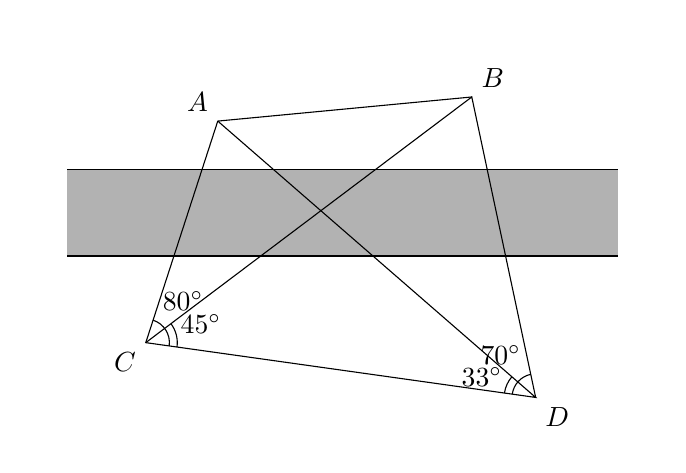
\begin{tikzpicture}
        \clip (-1.5,-1.3) rectangle (6.5,4);
        \fill [gray!60] (-1,1.1) rectangle (6,2.2);
        \draw (0,0) node [below left] {$C$} coordinate (C) ++ (-8:5) node [below right] {$D$} coordinate (D);
        \path [name path = lineBC] (C) --++ (37:10);
        \path [name path = lineBD] (D) --++(102:10);
        \path [name intersections={of = lineBC and lineBD, by=B}];
        \draw (C) -- (B) node [above right] {$B$} --(D);
        \path [name path = lineAC] (C) --++ (72:10);
        \path [name path = lineAD] (D) --++(139:10);
        \path [name intersections={of = lineAC and lineAD, by=A}];
        \draw (B) -- (A) -- (C) -- (D) -- (A) node [above left] {$A$};
        \draw (C) ++ (-8:0.3) arc (-8:72:0.3) node [above right] {$80^\circ$};
        \draw (C) ++ (-8:0.4) arc (-8:37:0.4) node [right] {$45^\circ$};
        \draw (D) ++ (172:0.4) arc (172:139:0.4) node [left] {$33^\circ$};
        \draw (D) ++ (172:0.3) arc (172:102:0.3) node [above left] {$70^\circ$};
        \draw (-1,1.1) -- (6,1.1) (-1,2.2) -- (6,2.2);
    \end{tikzpicture}
\end{center}
\item 在平行四边形$ABCD$中, 已知$AB=10\sqrt 3$, $B=60^\circ$, $AC=30$, 求平行四边形的面积.
\item 在$\triangle ABC$中, 已知$a=2\sqrt 3$, $B=45^\circ$, 面积$S=3+\sqrt 3$, 求$c$和$C$.
\item 已知$\triangle ABC$的面积$S=\dfrac{b^2+c^2-a^2}4$, 求$A$.
\item 在$\triangle ABC$中, 已知$A=30^\circ$, $b=18$, 分别根据下列条件求$B$.\\
(1) \textcircled{1} $a=6$; \textcircled{2} $a=9$; \textcircled{3} $a=13$; \textcircled{4} $a=18$; \textcircled{5} $a=22$;\\
(2) 根据上述计算结果, 讨论使$B$有一解、两解、无解时$a$的取值情况.
\item 在$\triangle ABC$中, 求证: $a\cos ^2\dfrac C2+c\cos ^2\dfrac A2=\dfrac 12(a+b+c)$.
\item 某船在海面$A$处测得灯塔$C$在北偏东$30^\circ$方向, 与$A$相距$10\sqrt 3$海量, 测得灯塔$B$在北偏西$75^\circ$方向, 在$A$相距$15\sqrt 6$海里. 船由$A$向正北方向航行到$D$处, 测得灯塔$B$在南偏西$60^\circ$方向.这时灯塔$C$与$D$相距多少海里? $C$在$D$的什么方向?
\item 如图, 自动卸货汽车采用液压机构, 设计时需要计算油泵顶杆$BD$的长度, 已知车厢的最大仰角为$60^\circ$, 油泵顶点$B$与车厢支点$A$之间的距离为$1.95$米, $AB$与水平线之间的夹角为$6^\circ 20'$, $AC$的长为$1.40$米, 计算$BC$的长(结果保留$3$个有效数字).
\begin{center}
    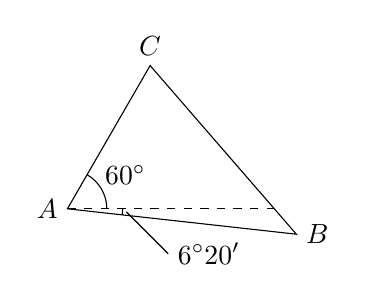
\begin{tikzpicture}[scale = 1.5]
        \draw (0,0) node [left] {$A$} coordinate (A);
        \draw (60:1.4) node [above] {$C$} coordinate (C);
        \draw ({-6-1/3}:1.95) node [right] {$B$} coordinate (B);
        \draw (A) -- (B) -- (C) -- cycle;
        \path [name path = dashedline] (A) --++ (1.9,0);
        \path [name path = BC] (B) -- (C);
        \path [name intersections = {of = dashedline and BC, by = D}];
        \draw [dashed] (A) -- (D);
        \draw (A) pic ["$60^\circ$",draw, angle eccentricity = 1.7] {angle = D--A--C};
        \draw (A) pic [draw, angle radius = 0.7cm] {angle = B--A--D};
        \draw (-3:0.5) --++ (-45:0.5) node [right] {$6^\circ 20'$};
    \end{tikzpicture}
\end{center}
\item 设计一个方案: 用测角仪与皮尺, 在上海延安东路外滩测量金茂大厦与东方明珠之间的距离.
\item 在平面直角坐标系中, 下列结论正确的是\bracket{20}.
\twoch{小于$\dfrac{\pi}2$的角一定是锐角}{第二象限的角一定是钝角}{始边相同且相等的角的终边一定相同}{始边相同, 终边也相同的角一定相等}
\item 当$0<\alpha <\dfrac{\pi}4$时, 化简$\sqrt {1-\sin 2\alpha}$的结果是\bracket{20}.
\twoch{$\cos \alpha$}{$\sin \alpha -\cos \alpha$}{$\cos \alpha -\sin \alpha$}{$\sin \alpha -\cos \alpha$或$\cos \alpha -\sin \alpha$}
\item 已知$\theta$为锐角, 则$\log _{\sin \theta}(1+\cot ^2\theta)=$\blank{50}.
\item 已知$\sin (\pi -\alpha)=\dfrac 23$, $\alpha \in (\dfrac{\pi}2,\pi)$, 则$\sin 2\alpha =$\blank{50}.
\item 如果某一电子钟的分针为$5\text{cm}$, 那么在$40$分钟内, 分针的端点转过的弧长为多少?
\item 已知圆$O$上的一段圆弧长等于该圆的内接正方形的边长, 求这段圆弧所对的圆心角的弧度数.
\item 在半径等于$10\text{cm}$的圆中, 一个圆中, 一个扇形的圆心角是$100^\circ$, 求这个扇形的周长和面积.
\item 已知角$\alpha$的终边经过点$P(3a,-4a)$($a\ne 0$), 求$\sin \alpha$、$\cos \alpha$和$\tan \alpha$的值.
\item 化简: $\dfrac{\sin (\theta -5\pi)}{\tan (3\pi -\theta)}\cdot \dfrac{\cot (\dfrac{\pi}2-\theta)}{\tan (\theta -\dfrac{3\pi}2)}\cdot \dfrac{\cos (8\pi -\theta)}{\sin (-\theta -4\pi)}$.
\item 化简: $\sin (\theta -\dfrac{\pi}4)+\cos (\theta +\dfrac{\pi}4)$.
\item 已知等式$\sqrt {\dfrac{1+\sin (\theta -\pi)}{1+\cos (\dfrac{\pi}2-\theta)}}=\tan (\theta +\pi)-\sec \theta$成立, 求$\theta$的取值范围.
\item 已知$\sin \alpha +\cos \alpha =\dfrac 23$, $\alpha \in (0,\pi)$, 求$\sin \alpha$、$\cos \alpha$的值.
\item 已知$\sin \alpha =\dfrac{\sqrt 5}5$, $\sin \beta =\dfrac{\sqrt {10}}{10}$, $\alpha$、$\beta$都是锐角, 求$\alpha +\beta$的值.
\item 求证: $\dfrac{2(\sin 2\alpha +1)}{1+\sin 2\alpha +\cos 2\alpha}=\tan \alpha +1$.
\item 已知$\angle A$、$\angle B$和$\angle C$是$\triangle ABC$的内角,
求证: $\tan \dfrac A2\cdot \tan \dfrac B2+\tan \dfrac B2\cdot \tan \dfrac C2+\tan \dfrac C2\cdot \tan \dfrac A2=1$.
\item (1)完成下表($\theta$为弧度数):
\begin{center}
    \begin{tabular}{|p{.05\textwidth}<{\centering}|p{.1\textwidth}<{\centering}|p{.1\textwidth}<{\centering}|p{.1\textwidth}<{\centering}|p{.1\textwidth}<{\centering}|p{.1\textwidth}<{\centering}|p{.1\textwidth}<{\centering}|p{.1\textwidth}<{\centering}|}
        \hline
        $\theta$ & $0.5$ & $0.4$ & $0.2$ & $0.1$ & $0.01$ & $0.001$ & $0.0001$\\ \hline
        $\sin \theta$ & $0.4794255$	& & & &	$0.0099998$ & & \\ \hline
        $\dfrac{\sin \theta}\theta$ & $0.9588511$	& & & &	$0.9999833$ & & \\ \hline
    \end{tabular}
\end{center}	
(2) 观察上表中的数据, 你能发现什么规律?
\item 已知$\pi <\alpha <\dfrac{3\pi}2$, $\pi <\beta <\dfrac{3\pi}2$, $\sin \alpha =-\dfrac{\sqrt 5}5$, $\cos \beta =-\dfrac{\sqrt {10}}{10}$, 求$\alpha -\beta$的值.
\item 已知$\sin \alpha =\alpha \sin \beta$, $b\cos \alpha =\alpha \cos \beta$, 且$\alpha$、$\beta$为锐角, 求证: $\cos \alpha =\sqrt {\dfrac{a^2-1}{b^2-1}}$.
\item 已知$\dfrac{3\pi}2<\alpha <2\pi$, 化简$\dfrac{\sqrt {1-\cos \alpha}+\sqrt {1+\cos \alpha}}{\sqrt {1-\cos \alpha}-\sqrt {1+\cos \alpha}}+\dfrac{\sqrt {1+\sin \alpha}}{\sqrt {1-\sin \alpha}}$.
\item 求证: $2\sin \alpha +\sin 2\alpha =\dfrac{2\sin ^3\alpha}{1-\cos \alpha}$.
\item 在$\triangle ABC$中, 求证:
(1)$\dfrac{\cos 2A}{a^2}-\dfrac{\cos 2B}{b^2}=\dfrac 1{a^2}-\dfrac 1{b^2}$.
(2)$(a^2-b^2-c^2)\tan A+(a^2-b^2+c^2)\tan B=0$.
\item 如图, 已知四边形$ABCD$的两条对角线$AC$与$BD$的夹角为$\theta$, 两条对角线长(同一长度单位)的乘积为$p$, 试用$p$和$\theta$表示四边形的面积$S$.
\item 在$\triangle ABC$中, $a=4$, $A=30^\circ$.\\
(1) 请你给出一个$b$值, 使该三角形有唯一解;\\
(2) 请你给出一个$b$值, 使该三角形有两解;\\
(3) 请你给出一个$b$值, 使该三角形无解.
\item 若$MP$和$OM$分别是角$\dfrac{7\pi}6$的正弦线和余弦线, 则\bracket{20}.
\fourch{$MP<OM<0$}{$OM>0>MP$}{$OM<MP<0$}{$MP>0>OM$}
\item 作出函数$y=1+\sin x, \ x\in [-\pi ,\pi]$的大致图像.
\item 作出函数$y=-\cos x,\ x\in [0,2\pi]$的大致图像.
\item 求函数$y=\dfrac 1{1+\sin x}$的定义域.
\item 求函数$y=\sqrt {-2\cos x}$的定义域.
\item 求函数$y=\cos x+3$的值域.
\item 求函数$y=4\sin ^2x-2$的值域.
\item 求函数$y=2-\sin x$取得最大值和最小值的$x$的集合, 并求出其最大值和最小值.
\item \item 求函数$y=3\sin (2x-\dfrac{\pi}3)$取得最大值和最小值的$x$的集合, 并求出其最大值和最小值.
\item 如图, 把一段直径$20$厘米的圆柱形木料截成横截面为矩形的木料, 怎样锯才能使横截面的面积最大?
\begin{center}
    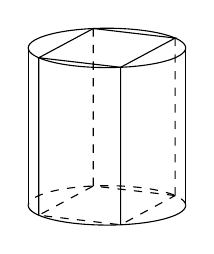
\begin{tikzpicture}
        \draw (0,2) ellipse (1 and 0.25);
        \draw (-1,0) arc (180:360:1 and 0.25);
        \draw [dashed] (1,0) arc (0:180:1 and 0.25);
        \draw (-1,0) -- (-1,2) (1,0) -- (1,2);
        \draw (0,0) ++ ({cos(30)},{0.25*sin(30)}) coordinate (A) ++ (0,2) coordinate (A1);
        \draw (0,0) ++ ({cos(100)},{0.25*sin(100)}) coordinate (B) ++ (0,2) coordinate (B1);
        \draw (0,0) ++ ({cos(210)},{0.25*sin(210)}) coordinate (C) ++ (0,2) coordinate (C1);
        \draw (0,0) ++ ({cos(280)},{0.25*sin(280)}) coordinate (D) ++ (0,2) coordinate (D1);
        \draw [dashed] (A) -- (B) -- (C) -- (D) --cycle (A) -- (A1) (B) -- (B1);
        \draw (A1) -- (B1) -- (C1) -- (D1) -- cycle (D) -- (D1) (C) -- (C1);
    \end{tikzpicture}
    \begin{tikzpicture}[>=latex]
        \path (0,2) ellipse (1 and 0.25);
        \path (-1,0) arc (180:360:1 and 0.25);
        \path [dashed] (1,0) arc (0:180:1 and 0.25);
        \path (-1,0) -- (-1,2) (1,0) -- (1,2);
        \draw [->] (-0.5,1) -- (0.5,1);
    \end{tikzpicture}    
    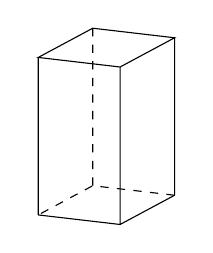
\begin{tikzpicture}
        \path (0,2) ellipse (1 and 0.25);
        \path (-1,0) arc (180:360:1 and 0.25);
        \path [dashed] (1,0) arc (0:180:1 and 0.25);
        \path (-1,0) -- (-1,2) (1,0) -- (1,2);
        \draw (0,0) ++ ({cos(30)},{0.25*sin(30)}) coordinate (A) ++ (0,2) coordinate (A1);
        \draw (0,0) ++ ({cos(100)},{0.25*sin(100)}) coordinate (B) ++ (0,2) coordinate (B1);
        \draw (0,0) ++ ({cos(210)},{0.25*sin(210)}) coordinate (C) ++ (0,2) coordinate (C1);
        \draw (0,0) ++ ({cos(280)},{0.25*sin(280)}) coordinate (D) ++ (0,2) coordinate (D1);
        \draw [dashed] (A) -- (B) -- (C)  (B) -- (B1);
        \draw (A1) -- (B1) -- (C1) -- (D1) -- cycle (D) -- (D1) (C) -- (C1) (A) -- (A1) (C) -- (D) -- (A);
    \end{tikzpicture}
\end{center}
\item 如图, 太阳光斜照地面, 光线与水平面所成的角为$\theta$, 长为$l$的竹竿与地面所成的角为$\alpha$.当$\alpha$为多少时, 竹竿的影子最长?
\begin{center}
    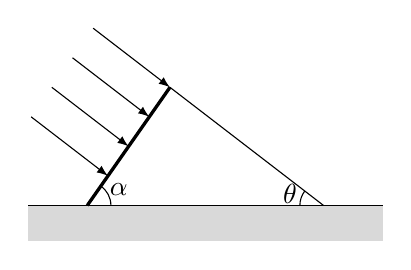
\begin{tikzpicture}[>=latex,scale = 1.5]
        \filldraw [gray!30] (-1.5,-0.3) rectangle (1.5,0);
        \draw (-1.5,0) -- (1.5,0);
        \draw [very thick] (-1,0) coordinate (A) -- (-0.3,1) coordinate (B);
        \draw (-0.3,1) -- (1,0) coordinate (C);
        \draw (A) pic ["$\alpha$", angle radius = 0.3cm, draw, angle eccentricity = 1.5] {angle = C--A--B};
        \draw (C) pic ["$\theta$", angle radius = 0.3cm, draw, angle eccentricity = 1.5] {angle = B--C--A};
        \draw ($(B)!0.25!(A)$) coordinate (B1) ++ (-0.65,0.5) coordinate (D1);
        \draw ($(B)!0.5!(A)$) coordinate (B2) ++ (-0.65,0.5) coordinate (D2);
        \draw ($(B)!0.75!(A)$) coordinate (B3) ++ (-0.65,0.5) coordinate (D3);
        \draw (B) ++ (-0.65,0.5) coordinate (D);
        \draw [->] (D) -- (B);
        \draw [->] (D1) -- (B1);
        \draw [->] (D2) -- (B2);
        \draw [->] (D3) -- (B3);
    \end{tikzpicture}
\end{center}
\item 求函数$y=\sin \dfrac x4$的周期.
\item 求函数$y=2\cos (2x+\dfrac{\pi}3)$的周期.
\item 求函数$y=\cos ^2x$的周期.
\item 求函数$y=\sin x+\sqrt 3\cos x$的周期.
\item 写出两个以$\dfrac{\pi}2$为周期的函数.
\item 已知函数$y=f(x)$的周期为$3$, 试求$y=f(2x+1)$的周期.
\item 判断函数$y=|\sin x|$的奇偶性, 并说明理由.
\item 判断函数$y=3\sin x+1$的奇偶性, 并说明理由.
\item 判断函数$y=\sin x+\sin 2x$的奇偶性, 并说明理由.
\item 判断函数$y=\sin ^2x+\cos 2x$的奇偶性, 并说明理由.
\item 求函数$y=\sin 2x$的单调递增区间.
\item 已知$0\le x\le 2\pi$, 求适合下列条件的角$x$的集合:\\
(1) 角$x$的正弦函数、余弦函数都是增函数;\\
(2) 角$x$的正弦函数是减函数, 余弦函数是增函数.
\item 作出函数$y=|\sin x|, \ x\in [\pi ,3\pi]$的大致图像.
\item 已知$\sin \alpha \ge \dfrac 12$, 试求$[0,2\pi]$中的$\alpha$的取值范围.
\item 函数$y=k\sin x+b$的最大值为$2$, 最小值为$-4$, 求$k$、$b$的值.
\item 求函数$y=\sqrt 3\sin x+\cos x$取得最大值和最小值的$x$的集合, 并求出其最大值和最小值.
\item 求函数$y=2+|\cos x|$取得最大值和最小值的$x$的集合, 并求出其最大值和最小值.
\item 求函数$y=\sin ^2x+2\sin x\cos x$的周期.
\item 求函数$y=\sin ^4x+\cos ^4x$的周期.
\item 如图所示, 函数$y=f(x)(x\in \mathbf{R})$的图像由折线段组成, 其中$x$取偶数时, 对应的$y$值为$0$; $x$到奇数时, 对应的$y$值为$2$.
\begin{center}
    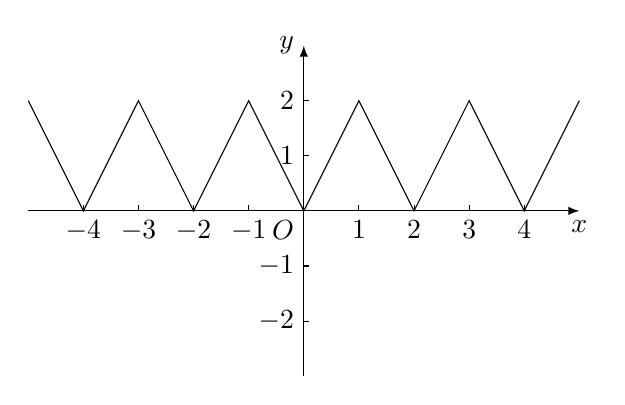
\begin{tikzpicture}[>=latex,scale = 0.7]
        \draw [->] (-5,0) -- (5,0) node [below] {$x$};
        \draw [->] (0,-3) -- (0,3) node [left] {$y$};
        \draw (0,0) node [below left] {$O$};
        \foreach \i in {-4,-3,-2,-1,1,2,3,4}
        {\draw (\i,0.1) -- (\i,0) node [below] {$\i$};};
        \foreach \i in {-2,-1,1,2}
        {\draw (0.1,\i) -- (0,\i) node [left] {$\i$};};
        \draw (-5,2) -- (-4,0) -- (-3,2) -- (-2,0) -- (-1,2) -- (0,0) -- (1,2) -- (2,0) -- (3,2) -- (4,0) -- (5,2);
    \end{tikzpicture}
\end{center}
(1) 写出函数$y=f(x)$的周期;\\
(2) 作出函数$y=f(x-1)$的图像.
\item 试写出一个满足条件$f(3\pi +x)=f(x)$且$f(-x)=-f(x)$的函数$y=f(x)$.
\item 试写出一个满足条件$f(x-4\pi)=f(x)$且$f(-x)-f(x)=0$的函数$y=f(x)$.
\item 求函数$y=\sin (\dfrac{\pi}6-x)$的递减区间.
\item 求函数$y=\tan \dfrac x2$的周期.
\item 求函数$y=\tan \pi x$的周期.
\item 求函数$y=\tan (2x-\dfrac{\pi}4)$的周期.
\item 求函数$y=\cot x-\tan x$的周期.
\item 判断函数$f(x)=-2\tan 3x$的奇偶性, 并说明理由.
\item 判断函数$f(x)=x\tan x$的奇偶性, 并说明理由.
\item 已知$0\le x\le 2\pi$, 求使角$x$的正弦函数、正切函数都是增函数的角$x$的集合.
\item 已知$0\le x\le 2\pi$, 求使角$x$的余弦函数是减函数, 正切函数是增函数的角$x$的集合.
\item 求函数$y=4\tan (\dfrac x2-\dfrac{\pi}5)$的定义域和单调区间.
\item 若$f(x)=\tan (x+\dfrac{\pi}4)$, 则$f(0)$、$f(-1)$、$f(1)$的大小关系是\blank{50}(用``<''号连接这三个数).
\item 已知$a\in (0,\dfrac{\pi}2)$, 比较$\alpha$、$\tan \alpha$、$\sin \alpha$的大小, 并利用三角函数线的相关知识加以证明.
\item 求函数$f(x)=\dfrac{2\tan \dfrac x2}{1-\tan ^2\dfrac x2}$的最小正周期.
\item 要得到函数$y=3\sin x$的图像, 只需要把函数$y=\sin x$的图像上的对应点的横坐标\blank{50}, 纵坐标\blank{50}.
\item 要得到函数, $y=\sin 4x$的图像, 只需要把函数$y=\sin x$的图像上的对应点的纵坐标\blank{50}, 横坐标\blank{50}.
\item 作出函数$y=\sin x\cdot \cos x$在长度为一个周期的闭区间上的大致图像.
\item 作出函数$y=2\sin \dfrac x2$在长度为一个周期的闭区间上的大致图像.
\item 作出函数$y=\sin (x-\dfrac{\pi}6)$在长度为一个周期的闭区间上的大致图像.
\item 作出函数$y=2\sin (x+\dfrac{\pi}3)$在长度为一个周期的闭区间上的大致图像.
\item 写出函数$y=3\sin (\dfrac x2+\dfrac{\pi}3)$的周期、振幅、初相、频率.
\item 已知函数$y=A\sin (\omega x+\varphi),(A>0,\omega >0)$的振幅是$3$, 最小正周期是$\dfrac{2\pi}7$, 初相是$\dfrac{\pi}6$, 求这个函数的解析式.
\item 一根细线的一端固定, 另一端悬挂一个小球, 小球来回摆时, 离开平衡位置的位移$s$(厘米)和时间$t$(秒)的函数关系是$s=6\sin (2\pi t+\dfrac{\pi}6)$.\\
(1) 小球开始摆动时, 离开平衡位置多少厘米?\\
(2) 小球摆动时, 离开平衡位置的最大距离是多少厘米?\\
(3) 小球来回摆动一次, 需要多少时间?
\item 设$y=f(t)$是某港口水的深度$y$(米)关于时间$t$(时)的函数, 其中$0\le t\le 24$, 下表是该港口某一天从$0$时至$24$时记录的时间$t$(时)与水深$y$(米)的关系:
\begin{center}
    \begin{tabular}{|c|c|c|c|c|c|c|c|c|c|}
        \hline
        $t$(时) & $0$ & $3$ & $6$ & $9$ & $12$ & $15$ & $18$ & $21$ & $24$ \\ \hline
        $y$(米)	& $13$ & $16.1$ & $13.1$ & $10.1$ & $12.9$ & $15.9$ & $12.9$ & $9.9$ & $13.1$ \\ \hline
    \end{tabular}
\end{center}
经长期观察, 函数$y=f(x)$的图像可以近似地看成函数$y=k+A\sin (\omega t+\varphi)$的图像.
下面的函数中, 最能近似表示表中数据间对应关系的函数$(t\in [0,24])$是\bracket{20}.
\fourch{$y=13+3\sin \dfrac{\pi}6t$}{$y=13+3\sin (\dfrac{\pi}6t+\pi)$}{$y=13+3\sin \dfrac{\pi}{12}t$}{$y=13+3\sin (\dfrac{\pi}{12}t+\dfrac{\pi}2)$}
\item 电流强度$I$随时间$t$的变化关系是$I=A\sin (\omega t+\varphi _0)$, 设$\omega =100\pi$(弧度/秒), $A=50$(安培), $\varphi _0=\dfrac{\pi}6$.\\
(1) 求电流强度$I$的变化周期和频率;\\
(2) 当$t=\dfrac 1{50}$(秒)时, 求电流强度$I$.
\item 求下列各式的值(用弧度制表示):\\
(1) $\arcsin \dfrac 12$;\\
(2) $\arccos (-\dfrac{\sqrt 2}2)$;\\
(3) $\arccos 1$;\\
(4) $\arctan (-\sqrt 3)$.
\item 求下列各式的值(精确到$0.0001$):\\
(1) $\arcsin 0.2672$;\\
(2) $\arcsin (-0.3322)$;\\
(3) $\arccos \dfrac{\sqrt 6-\sqrt 2}4$;\\
(4) $\arctan (2-\sqrt 3)$.
\item 用反三角函数的形式表示下列各式中的$x$:\\
(1) $\sin x=\dfrac{\sqrt 5}5,\ x\in [-\dfrac{\pi}2,\dfrac{\pi}2]$;\\
(2) $\sin x=\dfrac 17, \ x\in [\dfrac{\pi}2,\pi]$;\\
(3) $\cos x=\dfrac 34, \ x\in [0,\pi]$;\\
(4) $\cos x=-\dfrac{\sqrt 5}5, \ x\in [-\pi ,0]$;\\
(5) $\tan x=\sqrt 3, \ x\in (-\dfrac{\pi}2,\dfrac{\pi}2)$;\\
(6) $\tan x=-\dfrac 23, \ x\in (\dfrac{\pi}2,\pi)$.
\item 求下列各式的值:\\
(1) $\sin (\arcsin \dfrac 14)$;\\
(2) $\cos [\arccos (-\dfrac{\sqrt 2}2)]$;\\
(3) $\tan (\arctan \dfrac 13)$;\\
(4)$\sin (\arccos \dfrac 45)$.
\item 求下列各式的值:\\
(1) $\arcsin (\sin 1)$;\\
(2) $\arcsin (\sin \dfrac{2\pi}3)$;\\
(3) $\arccos (\cos \dfrac{\pi}{12})$;\\
(4) $\arccos [\cos (-\dfrac{\pi}3)]$;\\
(5) $\arctan [\tan (-\dfrac{\pi}3)]$;\\
(6) $\arctan (\tan \dfrac{5\pi}4)$.
\item 某老城区在排地下管道时, 为了保护一棵古树, 需要重新安排管道走向, 现在要设计的管道如下图所示: 求管道切割的角度$\theta$和$\beta$的大小.(结果精确到$0.01$度)
\begin{center}
    \begin{tikzpicture}
        \draw (0,0) -- (3,0) coordinate (A) --++ (3,2.5) coordinate (B) --++ (3,0);
        \path [name path = line1] (A) --++ ({90+atan(2.5/3)/2}:0.8);
        \path [name path = horizontal1] (0,0.5) -- (4,0.5);
        \path [name intersections = {of = line1 and horizontal1, by = A1}];
        \path [name path = line2] (B) --++ ({90+atan(2.5/3)/2}:0.8);
        \path [name path = horizontal2] (4,3) -- (8,3);
        \path [name intersections = {of = line2 and horizontal2, by = B1}];
        \draw (A) -- (A1) (B) -- (B1);
        \draw (0,0) -- (0,0.5) coordinate (S) -- (A1) -- (B1) -- (9,3) coordinate (T) -- (9,2.5);
        \draw [dashed] (A1) -- ($(A1)!-2!(A)$) coordinate (A2) (B1) -- ($(B1)!-2!(B)$) coordinate (B2);
        \draw (A1) pic ["$\theta$", draw, angle eccentricity = 1.3] {angle = A2--A1--S};
        \draw (A1) pic ["$\theta$", draw, angle eccentricity = 1.3] {angle = B1--A1--A2};
        \draw (B1) pic ["$\beta$", draw, angle eccentricity = 1.3] {angle = T--B1--B2};
        \draw (B1) pic ["$\beta$", draw, angle eccentricity = 1.3] {angle = B2--B1--A1};
    \end{tikzpicture}
\end{center}
\item 求函数$y=\arcsin (x-1)$的定义域、值域.
\item 求函数$y=2\arccos (\dfrac 12-x)$的定义域、值域.
\item 求函数$y=\arctan \sqrt {x+1}$的定义域、值域.
\item 求$\tan (\arcsin \dfrac 45)$的值.
\item 求$\sin [\dfrac{3\pi}4+\arccos (-\dfrac{\sqrt 3}2)]$的值.
\item 求$\sin (\arcsin \dfrac 12+\arccos \dfrac{\sqrt 3}2)$的值.
\item 若$\sin \alpha =\dfrac{\sqrt {10}}{10}$, $\beta =\arccos (-\dfrac{\sqrt 5}5)$, $0<\alpha <\dfrac{\pi}2$, 求证: $\alpha +\beta =\dfrac{3\pi}4$.
\item 写出方程$\sin x=\dfrac{\sqrt 2}2$的解集:\blank{50}.
\item 写出方程$\sin x=-\dfrac 14$的解集:\blank{50}.
\item 写出方程$\cos x=-\dfrac{\sqrt 3}2$的解集:\blank{50}.
\item 写出方程$\cos x=\dfrac 15$的解集:\blank{50}.
\item 写出方程$\tan x=-1$的解集:\blank{50}.
\item 写出方程$\tan x=2$的解集:\blank{50}.
\item 求方程$\sin (x-\dfrac{2\pi}3)=\dfrac 12$的解集.
\item 求方程$\cos (5x+60^\circ)=\dfrac{\sqrt 3}2$的解集.
\item 求方程$\tan (\dfrac{\pi}4-x)=\dfrac{\sqrt 3}2$的解集.
\item 求方程$\cos (x+\dfrac{\pi}4)=\dfrac 12, \ x\in (0,2\pi)$的解集.
\item 求方程$3\tan (x+\dfrac{\pi}3)=\sqrt 3, \ x\in (0,\pi)$的解集.
\item 求方程$2\sin 2x-1=0, \ x\in (0,\dfrac{\pi}2)$的解集.
\item 求方程$3\sin ^2x+2\sin x-1=0$的解集.
\item 求方程$\sin \dfrac x2-\cos \dfrac x2=1$的解集.
\item 求方程$\sin 2x=-\dfrac 12$在$[0,2\pi)$上的解集.
\item 求方程$2\cos (3x+\dfrac{\pi}4)-\sqrt 2=0$在$[0,2\pi)$上的解集.
\item 求方程$3\tan (\dfrac x2-\dfrac{\pi}{12})=\sqrt 3$在$[0,2\pi)$上的解集.
\item 求方程$\sin x=\cos 2x$的解集.
\item 求方程$\sin x=2\sin (\dfrac{\pi}3-x)$的解集.
\item 设$MP$与$OM$分别是角$\dfrac{17}{18}\pi$的正弦线和余弦线, 则\bracket{20}.
\fourch{$MP<OM<0$}{$MP<0<OM$}{$OM<MP<0$}{$OM<0<MP$}
\item 函数$y=\sqrt 3\cos 2x-\sin 2x$的一个单调区间是\bracket{20}.
\fourch{$[-\dfrac{\pi}6,\dfrac{\pi}6]$}{$[\dfrac{\pi}6,\dfrac{2\pi}3]$}{$[\dfrac{\pi}{12},\dfrac{7\pi}{12}]$}{$[-\dfrac{\pi}{12},\dfrac{5\pi}{12}]$}
\item 使$\sin x=\dfrac{1+a}{1-a}$有意义的$a$的取值范围是\bracket{20}.
\fourch{$-1\le a<0$}{$0\le a<1$}{$a\le 0$}{$a\le 1$}
\item 为了得到函数$y=\sin (x-\dfrac{\pi}5)$的图像, 只需把函数$y=\sin x$上所有的点\bracket{20}.
\twoch{向右平衡$\dfrac{\pi}5$个单位长度}{向左平移$\dfrac{\pi}5$个单位长度}{向左平移$\dfrac{2\pi}5$个单位长度}{向右平移$\dfrac{2\pi}5$个单位长度}
\item 下列函数是奇函数的是\bracket{20}.\\
\textcircled{1} $y=\sin|x|$; \textcircled{2} $y=x\sin x$; \textcircled{3} $y=x\cos x$;  \textcircled{4} $y=x|\sin x|$.
\fourch{\textcircled{1}\textcircled{2}}{\textcircled{1}\textcircled{3}}{\textcircled{2}\textcircled{4}}{\textcircled{3}\textcircled{4}}
\item 函数$y=\dfrac 1{1-\tan x}$的定义域是\blank{50}.
\item 函数$y=2\tan x\cos x$的值域是\blank{50}.
\item 函数$y=2\cos ^2(2x+\dfrac{\pi}3)$的最小正周期是\blank{50}.
\item 函数$y=\cos (\pi x)$的单调递增区间是\blank{50}.
\item 函数$y=\arccos x(-1\le x\le 0)$的反函数是\blank{50}.
\item 作出$y=2\sin (x-\dfrac{\pi}4)+1$在区间$[-\pi ,\pi]$上的图像, 并写出它的振幅、周期、频率、初相、单词区间及值域.
\item 函数$y=a\sin x+b(a<0)$的最大值为$3$, 最小值为$3$, 求实数$a$和$b$的值.
\item 已知函数$f(x)=\cos ^2(\dfrac{\pi}2x)$, 求使$f(x+c)=f(x)$恒成立的最小正数$c$.
\item 已知函数$f(x)=2\cos (\dfrac{\pi}3-\dfrac x2)$, 求$y=f(x)$的单调递减区间和周期.
\item 解方程: $\tan x-\sqrt 3=0, \ x\in [-\pi ,\pi]$.
\item 解方程: $\sin 2x=\sin x, \ x\in [0,2\pi]$.
\item 求函数$f(x)=\cos x+\sin x, \ x\in [0,\pi]$的值域.
\item 已知$\sin \alpha =\dfrac 12$.\\
(1) 若$\alpha$为三角形的内角, 求$\alpha$;\\
(2) 若$\alpha$在第二象限, 求$\alpha$;\\
(3) 若$\alpha \in \mathbf{R}$, 求$\alpha$.
\item 已知函数$y=\dfrac 12a\cos x(\cos x+\sqrt 3\sin x)+1$, 且函数的图像过点$P(\dfrac{\pi}6,\dfrac 74)$.\\
(1) 求函数的解析式;\\
(2) 当$y$取最大值时, 求自变量$x$的集合.
\item 如图是某游乐场的摩天轮的示意图, 其最高点离地面$45$米, 直径为$40$米, 并以每$12$分钟一周的速度匀速旋转. 摩天轮上某个点$P$在$t=0$时位于最低点处. 求证: $P$离地面的高度$h$(米)与时间$t$(分)的函数关系是$h=-20\cos \dfrac{\pi}6t+25$.
\begin{center}
    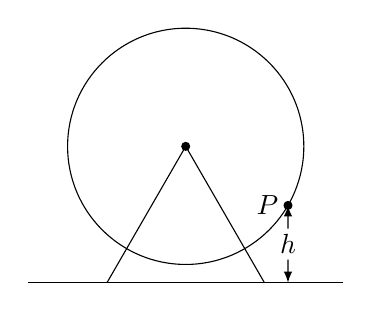
\begin{tikzpicture}[>=latex]
        \filldraw (0,0) circle (0.05);
        \draw (0,0) circle (1.5);
        \draw (0,0) -- (240:2) (0,0) -- (300:2);
        \draw (-2,{-sqrt(3)}) -- (2,{-sqrt(3)});
        \filldraw (330:1.5) circle (0.05) node [left] {$P$};
        \draw ({1.5*sqrt(3)/2},{-sqrt(3)}) coordinate (A)  (330:1.5) coordinate (B);
        \draw [->] ($(A)!0.3!(B)$) -- (A);
        \draw [->] ($(A)!0.7!(B)$) -- (B);
        \draw ($(A)!0.5!(B)$) node {$h$};
    \end{tikzpicture}
\end{center}
\item 弹簧挂着的小球作上下振动, 时间$t$(秒)与小球相对平衡位置(即静止时的位置)的高度$h$(厘米)之间的函数关系式是$h=2\sin (t+\dfrac{\pi}4)$, $t\in [0,+\infty)$.\\
(1) 小球开始振动时的位置在哪里?\\
(2) 小球最高点、最低点与平衡位置的距离分别是多少?\\
(3) 经过多少时间小球往复振动一次?\\
(4) 小球每$1$秒能往复振动多少次?
\item 若函数$y=\sin (\dfrac 12x+\varphi)$是偶函数, 则$\varphi$的一个值为\bracket{20}.
\twoch{$\varphi =-\pi$}{$\varphi =-\dfrac{\pi}2$}{$\varphi =-\dfrac{\pi}4$}{$\varphi =-\dfrac{\pi}8$}
\item 函数$y=\sin 2(x+\dfrac{5\pi}{12})$的单调递减区间为(以下$k\in \mathbf{Z}$)\bracket{20}.
\fourch{$[k\pi -\dfrac 23\pi , \ k\pi -\dfrac{\pi}6]$}{$[2k\pi +\dfrac 14\pi ,2k\pi +\dfrac{3\pi}4]$}{$[k\pi -\dfrac 16\pi , \ k\pi +\dfrac{\pi}3]$}{$(\dfrac{\pi}4,\dfrac{\pi}2)\cup (\dfrac{3\pi}4,\pi)$}
\item 函数$y=2\sin (3x-\dfrac{\pi}4)$的图像的两条相邻对称轴之间的距离为\bracket{20}.
\fourch{$\dfrac{\pi}3$}{$\dfrac{2\pi}3$}{$\pi$}{$\dfrac{4\pi}3$}
\item ``$a=1$''是``函数$y=\cos ^2ax-\sin ^2ax$的最小正周期为$\pi$''的\bracket{20}.
\twoch{充分不必要条件}{必要不充分条件}{充要条件}{既不充分也不必要条件}
\item 下列各式中正确的是\bracket{20}.
\twoch{$\arcsin (-\dfrac 12)=\arccos \dfrac{\sqrt 3}2$}{$\arccos (-\dfrac 12)=\arcsin \dfrac{\sqrt 3}2$}{$\arctan (-1)=\arcsin (-1)$}{$\arcsin (-\dfrac{\sqrt 2}2)+\arccos \dfrac{\sqrt 2}2=0$}
\item 函数$y=\sin (\dfrac{\pi}3-2x)+\sin 2x$的周期是\blank{50}.
\item 函数$y=\sin (x-\dfrac{\pi}6)$图像的一个对称中心是\blank{50}.
\item 方程$\cos 2x=\cos x$在$[0,2\pi]$内的解集为\blank{50}.
\item 函数$y=1+\sin x, \ x\in [-\pi ,2\pi]$的图像与直线$y=\dfrac 32$的交点个数是\blank{50}.
\item 已知下列四个命题:\\
\textcircled{1} 函数$y=\sin (\dfrac{5\pi}2-2x)$是偶函数;
\textcircled{2} 函数$y=\tan x$在定义域内是增函数;
\textcircled{3} 函数$y=\tan (ax-1)$的最小正周期是$\dfrac{\pi}a$;
\textcircled{4} $x=\dfrac{\pi}8$是函数$y=\sin (2x+\dfrac{\pi}4)$图像的一条对称轴方程.
其中正确命题的序号是\blank{50}.
\item 设函数$f(x)=b-k\cos (2x-\dfrac{\pi}3)(k>0)$的定义域是$[0,\dfrac{\pi}2]$, 值域是$[-5,1]$, 求常数$k$与$b$的值.
\item 设函数$y=f(x)$满足$f(x+2)=-f(x)$, 且$f(2)=2$, 求$f(-2)$、$f(4)$、$f(100)$的值.
\item 设方程$\sin x+\sqrt 3\cos x=a$在区间$(0,2\pi)$内有两个相异的实数根$x_1$、$x_2$, 求$a$的取值范围及$x_1+x_2$的值.
\item 已知一个矩形内接于半径为$R$的圆.\\
(1)当矩形周长最大时, 求其面积;\\
(2)当矩形面积最大时, 求其周长.
\item 从某地发射一颗卫星, 进入轨道后每$2$小时绕地球一周, 卫星轨道所在平面与赤道所在平面(天球赤道平面)的交线为$AB$.设卫星离$AB$距离为$y$(千米), 时间$t$以分钟为单位, 则$y=b\cos (\dfrac{t-h}a)$. 如果卫星发射进入轨道后经$15$分钟到达最北点, 该点离$AB$的距离为$45000$千米, 再经过$1$小时卫星到达最南点, 离$AB$的距离也是$45000$千米.
\begin{center}
    \begin{tikzpicture}[rotate = {-23-26/60}]
        \filldraw [gray!30] (0,0) ellipse (2 and 0.8);
        \draw (-2,0) arc (180:360:2 and 0.8);
        \draw [dashed] (-2,0) arc (180:0:2 and 0.8);
        \draw (0,0) circle (2);
        \filldraw (0,0) circle (0.5);
        \filldraw [fill = white, draw = black] (100:2) circle (0.08) node [above] {卫星};
        \draw (-2,0) node [left] {$A$} -- (2,0) node [right] {$B$};
        \draw (0,-2.5) -- (0,2.5);
        \draw (0,0.5) node [above right] {北极};
        \draw (0,-0.5) node [below left] {南极};
        \draw (1,-0.4) --++ (250:0.5) node [below] {赤道平面};
        \draw (0,0) -- (150:1) node [above] {地球};
        \draw (150:2) -- (150:2.5) node [above] {卫星轨道};
        \draw (80:2) -- (80:2.5) node [above] {天球};
    \end{tikzpicture}
\end{center}
(1) 求$a$、$b$、$h$的值;\\
(2) 发射进入轨道$1$小时后, 卫星离$AB$多远?
\item 如果已知$f(x)=2^{-x}$, 则$f(\log _23)=$\blank{50}.
\item 如果函数$y=f(x)$的图像经过第三、四象限, 那么函数$y=f^{-1}(x)$的图像经过第\blank{50}象限.
\item 若$\log _x\dfrac 45<1$, 则$x$的取值范围为\blank{50}.
\item 函数$y=\dfrac 1{\sqrt {\log _{\frac 12}(2-x)}}$的定义域是\blank{50}.
\item 方程$3\tan x-1=0$的解集是\blank{50}.
\item $26$英寸的自行车车轮直径为$66.04\text{cm}$.若某同学骑这种型号的自行车上学, 从家到学校的行程是$1.66\text{km}$, 则车轮转了约\blank{50}周($\pi$取$3.14$).
\item 求值: $(1+\tan 21^\circ)(1+\tan 22^\circ)(1+\tan 23^\circ)(1+\tan 24^\circ)=$\blank{50}.
\item 函数$y=\cos ^2x$单调递增区间为\blank{50}.
\item 在同一坐标系内作出的两个函数图像如图所示, 这两个函数为\bracket{20}.
\begin{center}
    \begin{tikzpicture}[>=latex]
        \draw [->] (-2,0) -- (2,0) node [below] {$x$};
        \draw [->] (0,-2) -- (0,2) node [left] {$y$};
        \draw (0,0) node [below left] {$O$};
        \draw [domain = -1:2] plot (\x,{pow(2,-\x)});
        \draw [domain = -1:2] plot ({-pow(2,-\x)},-\x);
        \draw (0,1) node [above right] {$1$};
        \draw (-1,0) node [below left] {$-1$};
    \end{tikzpicture}
\end{center}
\twoch{$y=a^x$和$y=\log _a(-x)$}{$y=a^x$和$y=\log _ax^{-1}$}{$y=a^{-x}$和$y=\log _ax^{-1}$}{$y=a^{-x}$和$y=\log _a(-x)$}
\item 若$0<x<\dfrac{\pi}4$, 且$\lg (\sin x+\cos x)=\dfrac 12(3\lg 2-\lg 5)$, 则$\cos x-\sin x$的值为\bracket{20}.
\fourch{$\dfrac{\sqrt 6}3$}{$\dfrac{\sqrt 3}2$}{$\dfrac{\sqrt {10}}5$}{$\dfrac{\sqrt 5}4$}
\item 函数$y=\cos 2x+3\sin x$的值域是\bracket{20}.
\fourch{$[-4,\dfrac{17}8]$}{$(-\infty ,-4)\cup (\dfrac{17}8,+\infty)$}{$[-4,4]$}{$(-\infty ,-4)\cup (4,+\infty)$}
\item 设三角方程$\cos x=-1$与$\sin 3x=0$的解集分别为$E$和$F$, 那么\bracket{20}.
\fourch{$E\subsetneqq F$}{$E\supsetneqq F$}{$E\cap F=\varnothing$}{$E=F$}
\item 解方程: $\log _3(x-1)=\log _9(x+5)$.
\item 解方程: $\log _2(9^x-5)=\log _2(3^x-2)+2$.
\item 化学中的pH表示物体的酸碱程度. 其定义为pH$=-1g[H^+]$, 这里的$[H^+]$为每升中氢离子的浓度. 求出下列物体的pH:\\
(1) 醋: $[H^+]\approx 6.3\times 10^{-3}$;\\
(2) 胡萝卜: $[H^+]\approx 1.0\times 10^{-5}$;\\
(3) 已知海水的pH为$8.3$, 求海水的氢离子的浓度.
\item 已知函数$f(x)=\log _2(2^x-1)$.\\
(1) 求$f(x)$的定义域;\\
(2) 判断$f(x)$的增减性, 说明理由;\\
(3) 求$f^{-1}(x)$.
\item 设$a\in [0,2\pi]$, 比较 $\sin \alpha$与$\cos \alpha$的大小.
\item 已知$\tan \alpha =3$, 求$\dfrac 1{\sin ^2\alpha +2\sin \alpha \cos \alpha}$的值.
\item 已知函数$f(x)=a+b\cos 4x(b>0)$的最大值为$6$, 是小值为$-2$, 试求函数$y=b\cos \dfrac{\pi}ax$的周期和最值.
\item 若$0<a<\dfrac{\pi}2<\beta <\pi$, 且$\cos \beta =-\dfrac 13$, $\sin (\alpha +\beta)=\dfrac 79$, 求$\sin \alpha$的值.
\item 已知$\tan \alpha =\dfrac 17$, $\sin \beta =\dfrac{\sqrt {10}}{10}$, $\alpha, \beta \in (0, \dfrac{\pi}2)$, 求$\alpha +2\beta$.
\item 已知$-\dfrac{\pi}2<x<0$, $\sin x+\cos x=\dfrac 15$.\\
(1) 分别求$\sin x\cdot \cos x$与$\sin x-\cos x$的值;\\
(2) 求$\dfrac{3\sin ^2\dfrac x2-2\sin \dfrac x2\cos \dfrac x2+\cos ^2\dfrac x2}{\tan x+\cot x}$的值.
\item 证明: $(\sin \alpha +\sin \beta)^2+(\cos \alpha +\cos \beta)^2=4\cos ^2\dfrac{\alpha -\beta}2$.
\item 在$\triangle ABC$中, 已知$\sin A=\cos B\cos C$, 求证: $\tan B+\tan C=1$.
\item 已知函数$y=f(x)$的图像过点$A(1,2)$, 函数$y=g(x)$的图像与$y=f(x)$的图像关于直线$y=x$对称, 则$y=g(x)$的图像必过点\bracket{20}.
\fourch{$(2,1)$}{$(1,2)$}{$(-2,1)$}{$(-1,2)$}
\item 若$\log_m 3<\log_n 3<0$, 则$m,n$满足的条件是\bracket{20}.
\fourch{$m>n>1$}{$n>m>1$}{$0<m<n<1$}{$0<n<m<1$}
\item 若$\log _3x=\cos x$解的个数有\bracket{20}.
\fourch{$0$}{$1$}{$2$}{$3$}
\item 已知函数$f(x)=\cos \dfrac{\pi}2x$, 则下列等式成立的是\bracket{20}.
\fourch{$f(2\pi-x)=f(x)$}{$f(2\pi+x)=f(x)$}{$f(-x)=f(x)$}{$f(\pi-x)=f(x)$}
\item 若$\lg a\lg b$是方程$2x^2-4x+1=0$的两个根, 则$(\lg \dfrac ab)^2$的值等于\blank{50}.
\item 定义在$\mathbf{R}$上的偶函数$f(x)$在$[0,+\infty)$上是增函数, 且$f(\dfrac 12)=0$, 则满足$f(\log _{\dfrac 14}x)>0$的$x$的值范围是\blank{50}.
\item 在$\triangle ABC$中, 已知$a^2+b^2+ab=c^2$, 则$C=$\blank{50}.
\item 已知函数$f(x)=\log _a\dfrac{x+b}{x-b}(a>0,b>0a\ne 1)$.\\
(1) 求$f(x)$的定义域;\\
(2) 判断$f(x)$的奇偶性;\\
(3) 求函数$y=f^{-1}(x)$的解析式.
\item 已知$\alpha$是第二象限角, 且$\sin \alpha =\dfrac{\sqrt {15}}4$, 求$\dfrac{\sin (\alpha +\dfrac{\pi}4)}{\sin 2\alpha +\cos 2\alpha +1}$的值.
\item 在$\triangle ABC$中, 已知$(a^2+b^2)\sin (A-B)=(a^2-b^2)\sin C$, 试判断三角形的形状.
\item 在$\triangle ABC$中, 已知$C=2B$, 求证: $c^2-b^2=ab$.
\item 如图, $AB$为半圆$O$的直径, 点$P$在$AB$延长线上, 点$Q$在半圆上, 以$PQ$为一边作等边三角形$PQN$, 使$\triangle PQN$和$\triangle PQO$在$PQ$的两侧, 已知半圆的半径是$1$, $OP=2$.求四边形$OPNQ$的面积的最大值, 并求使四边形$OPNQ$面积取得最大值的$\angle QOP$的大小.
\begin{center}
    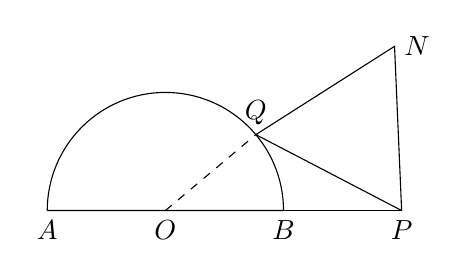
\begin{tikzpicture}[scale = 1.5]
        \draw (-1,0) node [below] {$A$} coordinate (A) -- (1,0) node [below] {$B$} coordinate (B) arc (0:180:1);
        \draw (0,0) node [below] {$O$} coordinate (O);
        \draw (B) -- (2,0) node [below] {$P$} coordinate (P);
        \draw (40:1) node [above] {$Q$} coordinate (Q);
        \draw ($(P)!1!-60:(Q)$) node [right] {$N$} coordinate (N);
        \draw [dashed] (O) -- (Q);
        \draw (P) -- (Q) -- (N) -- cycle;
    \end{tikzpicture}
\end{center}
\item 设在海拔$x$米处的大气压强是$y$帕, $y$与$x$之间的函数关系式是$y=ce^{kx}$, 其中$c,k$为常量.已知某地某天在海平面的大气压强为$1.01\times 10^5$帕, $1000$米高空的大气压强为$0.90\times 10^5$帕, 求$600$米高空的大气压强(结果保留$3$个有效数字)。


\end{enumerate}
\end{document}